\documentclass[11pt,a4paper]{article}
\usepackage{fontspec}
\setmainfont{TeX Gyre Pagella}
\newfontfamily\headfont{Inter}[UprightFont=*-ExtraBold,BoldFont=*-ExtraBold,Extension=.otf,Path=/usr/share/fonts/opentype/inter/]
\usepackage[a4paper,margin=2.3cm]{geometry}
\usepackage{graphicx,booktabs,float,caption,array,xcolor,longtable}
\usepackage[hidelinks]{hyperref}
\usepackage{titlesec}
\usepackage[round]{natbib}
\usepackage{setspace}
\setstretch{1.05}
\renewcommand{\topfraction}{0.9}
\renewcommand{\bottomfraction}{0.8}
\renewcommand{\textfraction}{0.1}
\renewcommand{\floatpagefraction}{0.75}
\setlength{\parindent}{0pt}
\setlength{\parskip}{0.55em}
\titleformat{\section}{\headfont\Large}{\thesection}{0.8em}{}
\titleformat{\subsection}{\headfont\large}{\thesubsection}{0.8em}{}
\captionsetup{font=small,labelfont=bf}
\urlstyle{same}
\hypersetup{pdftitle={Where the Borders Are Straight},pdfauthor={Tristan Hotham}}

\begin{document}
\begin{center}
{\Large\bfseries Where the Borders Are Straight\par}
\vspace{0.4em}
{\large Ruler lines, rivers and mountains on every international land border,\\and who drew the longest straight lines\par}
\vspace{1.2em}
{\large Tristan Hotham\par}
\vspace{0.3em}
{\small Independent researcher\\
ORCID: 0000-0003-4931-9349\\
DOI: \href{https://doi.org/10.5281/zenodo.23847974}{https://doi.org/10.5281/zenodo.23847974}\par}
\vspace{0.8em}
2026
\end{center}

\begin{quote}
\small
\begin{center}\textbf{Abstract}\end{center}
I classify every international land border in Natural Earth's 1:10 million boundary lines, 233,534 km between 170 countries and territories, into ruler-straight stretches, rivers and lakes, mountains and other lines, using an explicit geometric test for straightness (every vertex within 1 km of a great circle or rhumb line over at least 50 km), Natural Earth rivers and lakes, and the ETOPO5 elevation grid. 19.4\% of the world's land border length is straight, 20.9\% follows water and 24.7\% runs through mountains. Africa holds 53.8\% of all straight border length and the largest share of mostly straight borders, but by share of length North America (45.9\%) is straighter than Africa (30.2\%) under all 12 sensitivity settings, largely because of the border between Canada and the United States. For the 40 longest straight segments I compile, from published sources, the agreement that set each line, its year and the powers involved: 21 of 40 dated lines were set between 1880 and 1914, and the United Kingdom was party to 21. Straightness depends strongly on map scale: the same method finds 25.4\% straight on the 1:50 million lines and 83.6\% on the 1:110 million lines.

\textbf{Keywords:} international boundaries; borders; geometric boundaries; Africa; colonialism; treaties; cartographic generalisation; Natural Earth
\end{quote}

\section{Introduction}
Straight borders are among the most recognisable features of the political map, and among the most argued about. In Africa they are a shorthand for the Scramble: a continent divided in European capitals with a ruler and a coarse map. Political scientists and economists have used straight borders as a measure of how artificial a state is \citep{alesina2011} and colonial borders as a natural experiment \citep{michalopoulos2016}; historians of the boundaries themselves have documented the treaties line by line \citep{brownlie1979,biger1995,prescott2008}. Popular accounts go further and say Africa's borders are the straightest in the world, sometimes with a figure attached: that 44\% of them follow parallels and meridians, a number usually traced to \citet{barbour1961}.

This paper measures the straightness of every international land border with one transparent method and an open dataset, and asks four questions. How much of the world's border is straight, and how much follows rivers and mountains instead? Where are the straight borders, by continent and by country? Is Africa the straightest continent? And who drew the longest straight lines, and when? An interactive companion (\url{https://maps.tristanhotham.com/straight-borders/}) shows every border by kind with its treaty where known.

\section{Data}
\subsection{Borders}
The borders are Natural Earth's 1:10 million admin-0 land boundary lines \citep{naturalearth}, version 5.2.0-pre. I keep lines classed as international boundaries, disputed, indefinite, lines of control and indeterminate frontiers, and leave out overlay limits (UN buffer zones and demilitarised zones, which lie on top of other lines), lease limits (Guantanamo, Baikonur) and lines to zones rather than countries. This leaves 233,534 km in 332 borders, a border being the line between one pair of countries. Disputed, indefinite and ceasefire lines are 4.6\% of the length. Natural Earth draws borders as they exist in practice, which is not a judgement on any claim, and treats some entities separately (Western Sahara, Somaliland, Northern Cyprus, Palestine, Kosovo). The lines include stretches through lakes and estuaries, some marked by Natural Earth as water boundaries. The 1:50 million and 1:110 million versions of the same lines are used only to test the effect of map scale.

\subsection{Rivers, lakes, mountains and elevation}
Rivers are Natural Earth's 1:10 million river and lake centre lines with its supplementary European and North American rivers; lakes are its lakes with the same supplements. Elevation is ETOPO5 \citep{etopo5}, a 5 arc-minute (about 9 km) global grid, in the copy distributed with the Ferret datasets. Natural Earth's named physical regions supply 222 mountain ranges, used as an independent check.

\subsection{Treaties}
The table of treaties for the longest straight segments is compiled by hand from \citet{brownlie1979} for Africa, \citet{biger1995} and the US Department of State's International Boundary Study series elsewhere, the judgment of the International Court of Justice on the Libya and Chad boundary \citep{icj1994}, the boundary commissions of Canada, the United States and Mexico, and the English Wikipedia articles on each border, cross-checked where possible. It is published as data so that it can be corrected.

\section{Methods}
\subsection{Ruler-straight}
A border is a sequence of vertices. Starting at vertex $i$, I extend a candidate run to vertex $j$ for as long as every intermediate vertex lies within a tolerance $\tau$ of either the great circle through $i$ and $j$ or the rhumb line (a line of constant bearing, straight in the Mercator projection) through them, and the length along the border is at most 1\% more than the chord plus $\tau$, which stops a run from doubling back. If the run reaches at least $L$ km it is a straight segment and the search resumes at its end; otherwise it resumes at $i+1$. Both reference lines are needed: meridians are great circles, but parallels are rhumb lines and not great circles, and over 2,000 km the 49th parallel departs from a great circle by tens of kilometres. The main settings are $\tau = 1$ km and $L = 50$ km. A segment is a parallel if its latitude varies by less than $\tau$, a meridian if its longitude does, and otherwise a straight line between two points.

Natural Earth gives straight treaty lines many vertices (only 5 edges in the whole 1:10 million file are longer than 50 km), so a long run is evidence of a line drawn straight, not an artefact of sparse vertices. Lines that Natural Earth marks as water boundaries are classed as water even where drawn as straight courses, because the straight courses there only join turning points in the water; the courses through the Great Lakes are not so marked, and count as straight.

\subsection{Rivers and lakes}
Each border is resampled every kilometre. A sample follows water if it lies within 3 km of a river centre line or lake shore (computed from points every 0.5 km along them), inside a lake, or on a water boundary. Gaps of up to 3 km are filled and runs shorter than 15 km dropped, so that a border crossing a river does not count as following it.

\subsection{Mountains}
I first tried a direct crest test: is the border higher than the mean elevation 8 to 20 km away on both sides? On a 9 km grid this found crests on only a small part of borders well known to follow the Andes, Alps and Himalaya, because the grid smooths narrow crests and because watershed borders often run along plateau edges rather than the highest ground. I therefore classify terrain instead, with a simplified version of the UNEP-WCMC mountain definition \citep{kapos2000}: a sample is in mountains if ETOPO5 gives at least 2,500 m, or at least 300 m with a local elevation range of at least 300 m within a radius of two grid cells (about 18 km north to south). Gaps up to 3 km are filled and runs shorter than 20 km dropped. The class means \emph{through mountains}; most such borders follow crests or watersheds, but this method cannot say which. As a check, 59.1\% of mountain-class length lies inside a Natural Earth named mountain range, against 9.1\% of straight, 8.6\% of water and 13.3\% of other length.

\subsection{Priority, continents and countries}
Each kilometre takes the first class that applies, in the order straight, water, mountains, other. Borders are assigned to the continent Natural Earth gives both countries; borders between continents are placed where they lie (Russia's borders with Asian countries in Asia, Sinai and Gaza in Asia, Ceuta and Melilla in Africa, French Guiana in South America, New Guinea in Oceania, Panama and Colombia in North America). Country totals count every border of the country in full.

\subsection{Sensitivity}
I repeat the straightness test for $\tau \in \{0.25, 0.5, 1, 2\}$ km and $L \in \{25, 50, 100\}$ km, the water test for distances of 1.5, 3 and 5 km and minimum runs of 10, 15 and 30 km, and the mountain test for relief thresholds of 200, 300 and 500 m and radii of one to three cells; and I apply the straightness test with the main settings to the 1:50 million and 1:110 million lines.

\section{Results}
\subsection{The world's borders by kind}
Of 233,534 km of land border, 45,232 km (19.4\%) is straight, 48,871 km (20.9\%) follows rivers and lakes, 57,794 km (24.7\%) runs through mountains and 81,637 km (35.0\%) is other (Figure~\ref{fig:map}). The 312 straight segments are 20.6\% parallels, 15.6\% meridians and 63.8\% other straight lines; parallels and meridians together are 7.0\% of all border length. 47 of 332 borders (14.2\%) are at least half straight. Without disputed, indefinite and ceasefire lines the straight share is 19.1\%.

\begin{figure}[tbp]\centering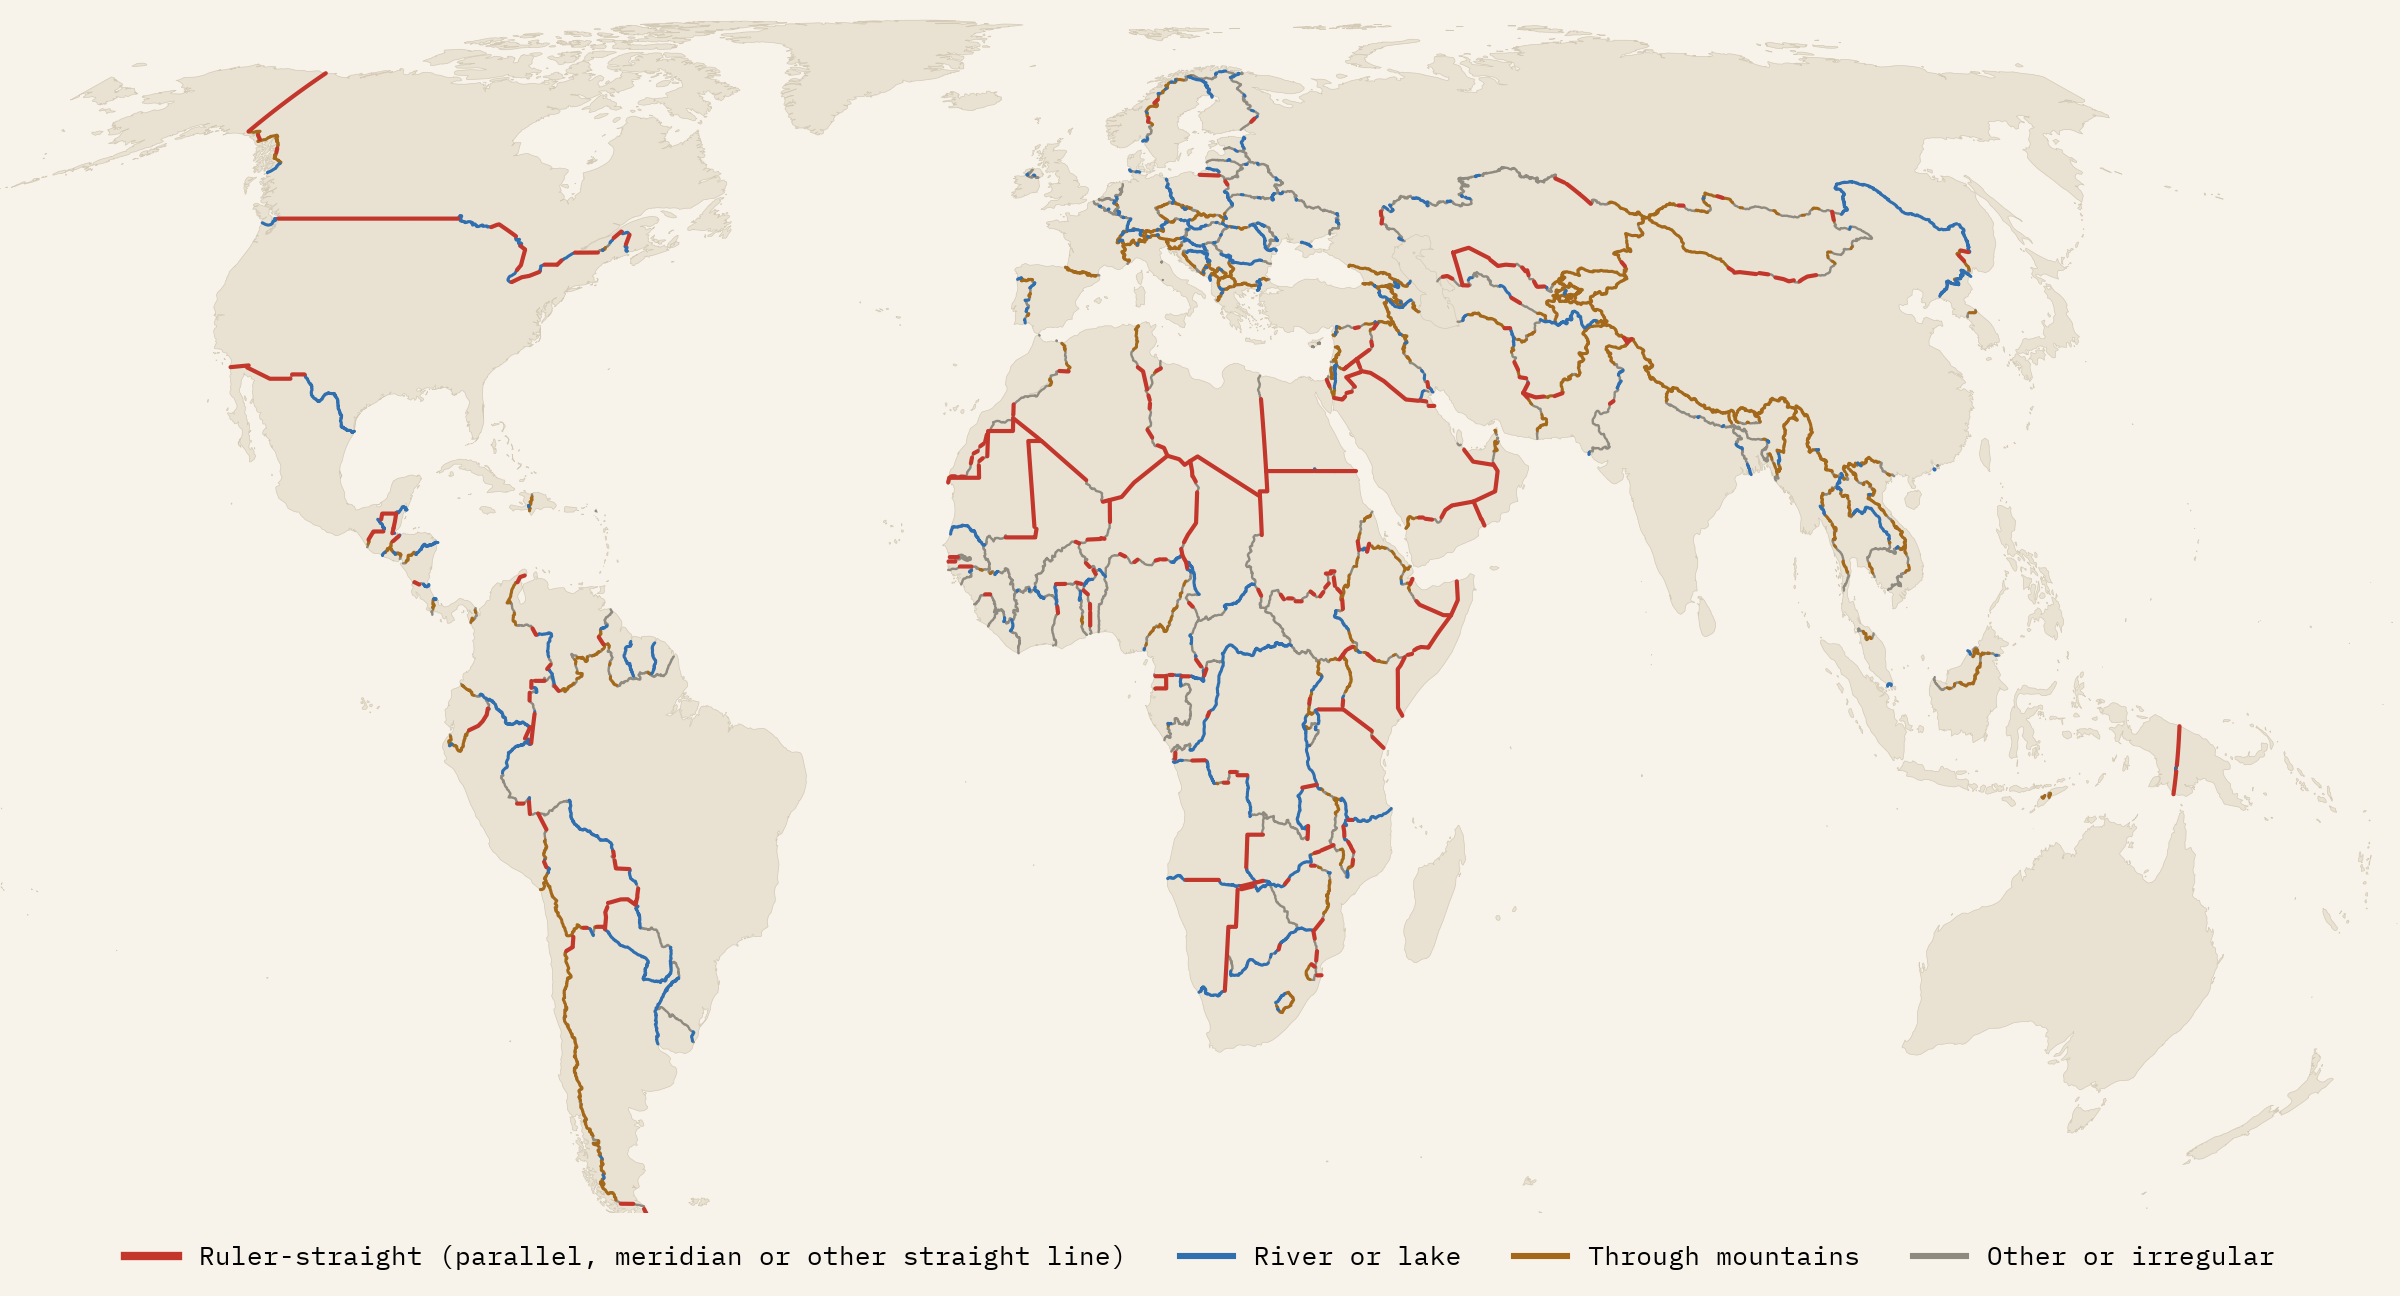
\includegraphics[width=\textwidth]{f_map.png}
\caption{Every international land border in Natural Earth's 1:10 million lines, by kind. Equal Earth projection.}\label{fig:map}\end{figure}

\subsection{By continent}
The continents differ sharply (Figure~\ref{fig:cont}, Table~\ref{tab:cont}). Europe's borders are almost never straight (1.5\%); Asia's run mostly through mountains (41.7\%); South America's follow rivers (31.3\%) and mountains (27.4\%). Oceania has a single land border, between Indonesia and Papua New Guinea, 87.9\% straight. Among the other five, North America is the straightest (45.9\%) and Africa second (30.2\%).

\begin{table}[tbp]\centering\small\caption{Land borders by continent: number of borders, length and share of length by kind (\%); parallels and meridians as a share of length; and the share of borders at least half straight.}\label{tab:cont}\setlength{\tabcolsep}{4pt}\begin{tabular}{lrrrrrrrr}\toprule Continent & Borders & km & Straight & Water & Mountain & Other & Par./mer. & Mostly straight\\\midrule
Oceania & 1 & 749 & 87.9 & 12.1 & 0.0 & 0.0 & 87.9 & 100.0\\
North America & 14 & 14,965 & 45.9 & 33.6 & 14.7 & 5.7 & 27.4 & 21.4\\
Africa & 110 & 80,457 & 30.2 & 20.5 & 8.5 & 40.7 & 12.3 & 25.5\\
South America & 25 & 29,934 & 13.2 & 31.3 & 27.4 & 28.1 & 3.2 & 4.0\\
Asia & 93 & 77,037 & 11.7 & 13.4 & 41.7 & 33.1 & 0.9 & 14.0\\
Europe & 89 & 30,392 & 1.5 & 24.7 & 27.5 & 46.3 & 0.0 & 1.1\\
\midrule World & 332 & 233,534 & 19.4 & 20.9 & 24.7 & 35.0 & 7.0 & 14.2\\
\bottomrule\end{tabular}\end{table}

\begin{figure}[tbp]\centering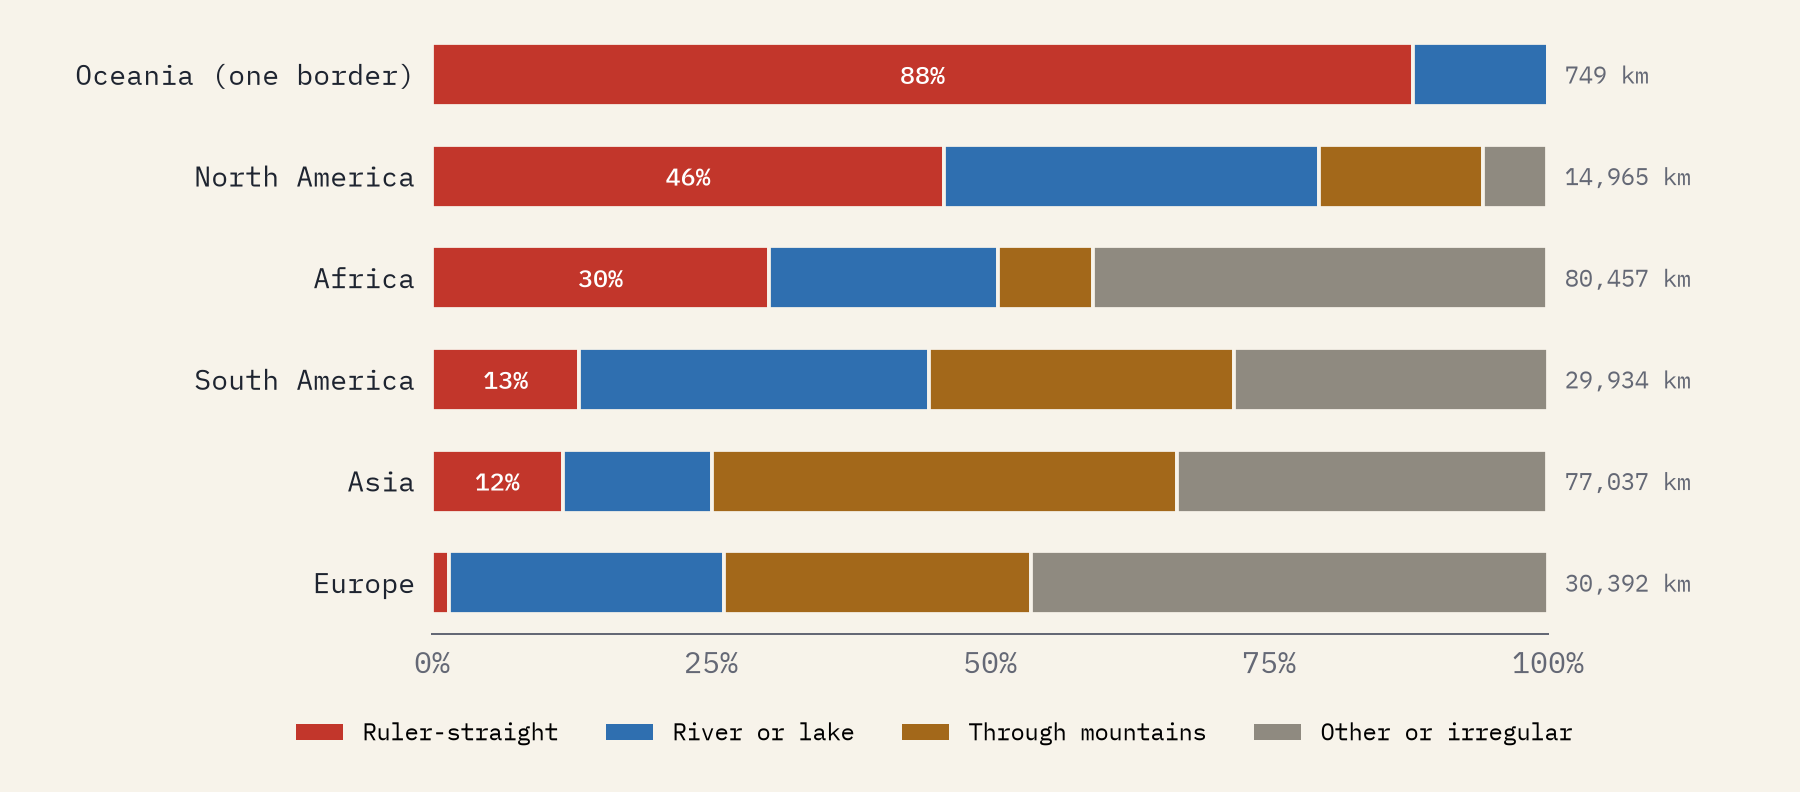
\includegraphics[width=.9\textwidth]{f_continents.png}
\caption{Share of each continent's land border length by kind.}\label{fig:cont}\end{figure}

\subsection{Is Africa the straightest?}
On three measures Africa leads. It has the most straight border, 24,332 km or 53.8\% of the world's; 25 of the 40 longest straight segments; and, among continents with more than one border, the largest share of borders that are at least half straight (25.5\%, against 21.4\% in North America). On the share of length it does not: North America is straighter under every one of the 12 settings tested (Figure~\ref{fig:sens}), with Africa second each time. The North American figure rests heavily on one border: Canada and the United States, 59.3\% straight over 8,352 km, which holds 72.2\% of the continent's straight length. Without it North America is 28.9\% straight, slightly below Africa. The popular claim is therefore right about quantity and wrong about proportion: most of Africa's border length (40.7\% other, 20.5\% water) is not straight. Parallels and meridians are 12.3\% of Africa's border length, well below the 44\% often quoted from \citet{barbour1961}; that study covered tropical Africa on maps of its time with its own categories, so the figures are not strictly comparable.

\begin{figure}[tbp]\centering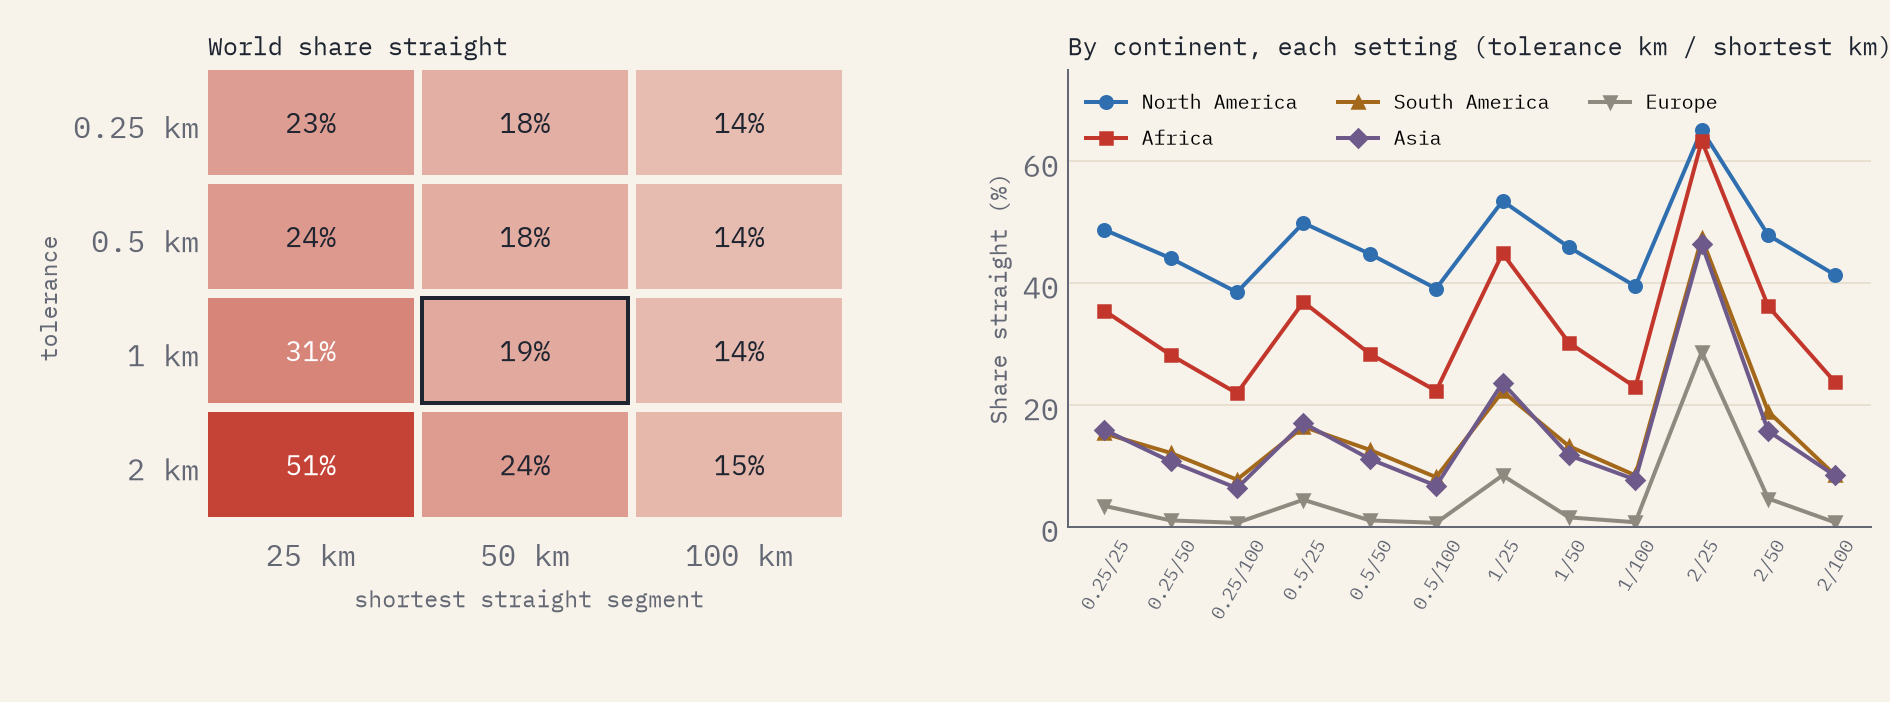
\includegraphics[width=\textwidth]{f_sens.png}
\caption{Sensitivity of the straight share to the tolerance and minimum segment length. Left: world share (main setting outlined). Right: share by continent at each setting (Oceania, one border, omitted).}\label{fig:sens}\end{figure}

\begin{figure}[tbp]\centering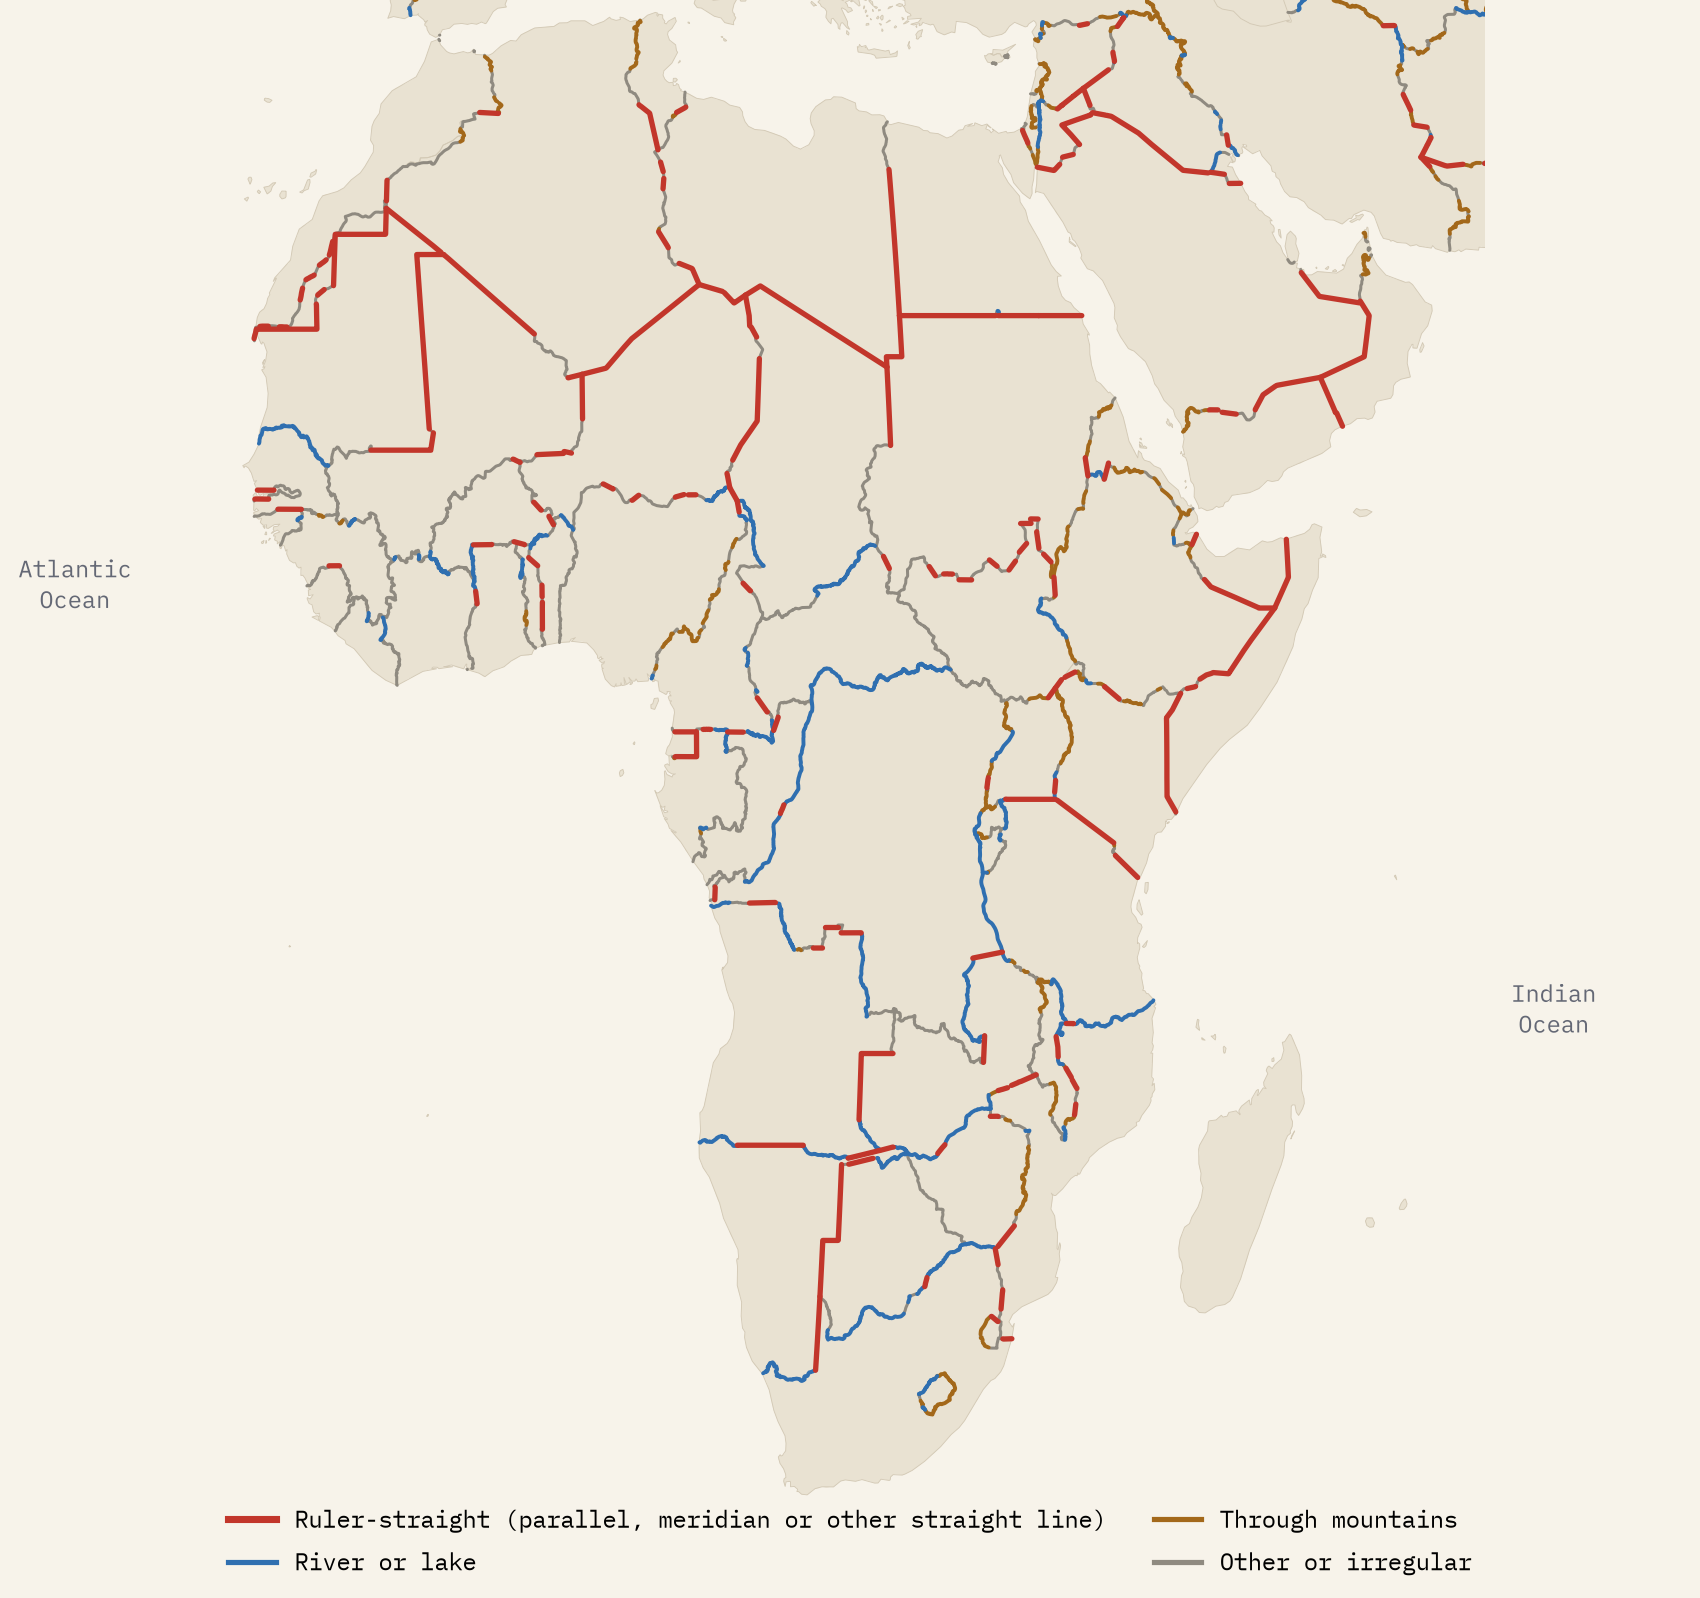
\includegraphics[width=.82\textwidth]{f_africa.png}
\caption{Africa and Arabia, borders by kind.}\label{fig:africa}\end{figure}

\subsection{By country}
Among countries with at least 1,000 km of land border, the straightest are Somalia (93.4\%), Egypt (80.7\%), Somaliland (79.7\%), Saudi Arabia (79.3\%) and Mauritania (71.1\%). 78 of 170 countries and territories have no straight border; 20 have at least half. The full table is in the data.

\subsection{The longest straight lines and who drew them}
Table~\ref{tab:top} and Figure~\ref{fig:top} list the 40 longest straight segments, which together make 40.7\% of all straight length. The longest is the 49th parallel between Canada and the United States (2,020 km), set by the Convention of 1818 east of the Rocky Mountains and the Oregon Treaty of 1846 west of them; then the 141st meridian between Alaska and Yukon (1,042 km, Anglo-Russian Convention of 1825); the line between Mali and Mauritania (945 km); the line between Libya and Chad (812 km), from the Anglo-French Declaration of 1899 as interpreted in 1919 and upheld by the International Court of Justice in 1994; and the 25th meridian between Egypt and Libya (803 km, 1925). The 22nd parallel between Egypt and Sudan (Condominium Agreement, 1899) is split into three segments by the disputed Hala'ib section, 1,212 km in all.

Of 40 dated lines, 6 were set before 1880, all in North America; 21 between 1880 and 1914, making up 47.0\% of the length of the 40; 9 between 1915 and 1945; and 4 after 1945, three in Arabia and the provisional line between Ethiopia and Somalia (Figure~\ref{fig:time}). The median year is 1899. The United Kingdom was a party to 21 lines, France to 11, Germany to 6 and Italy to 4. Several Saharan lines were not treaties between powers at all but limits France drew between its own colonies, confirmed as international borders by treaties between the independent states in the 1960s and 1980s. I rate 21 attributions high confidence, 18 medium and 1 low.

\begin{figure}[tbp]\centering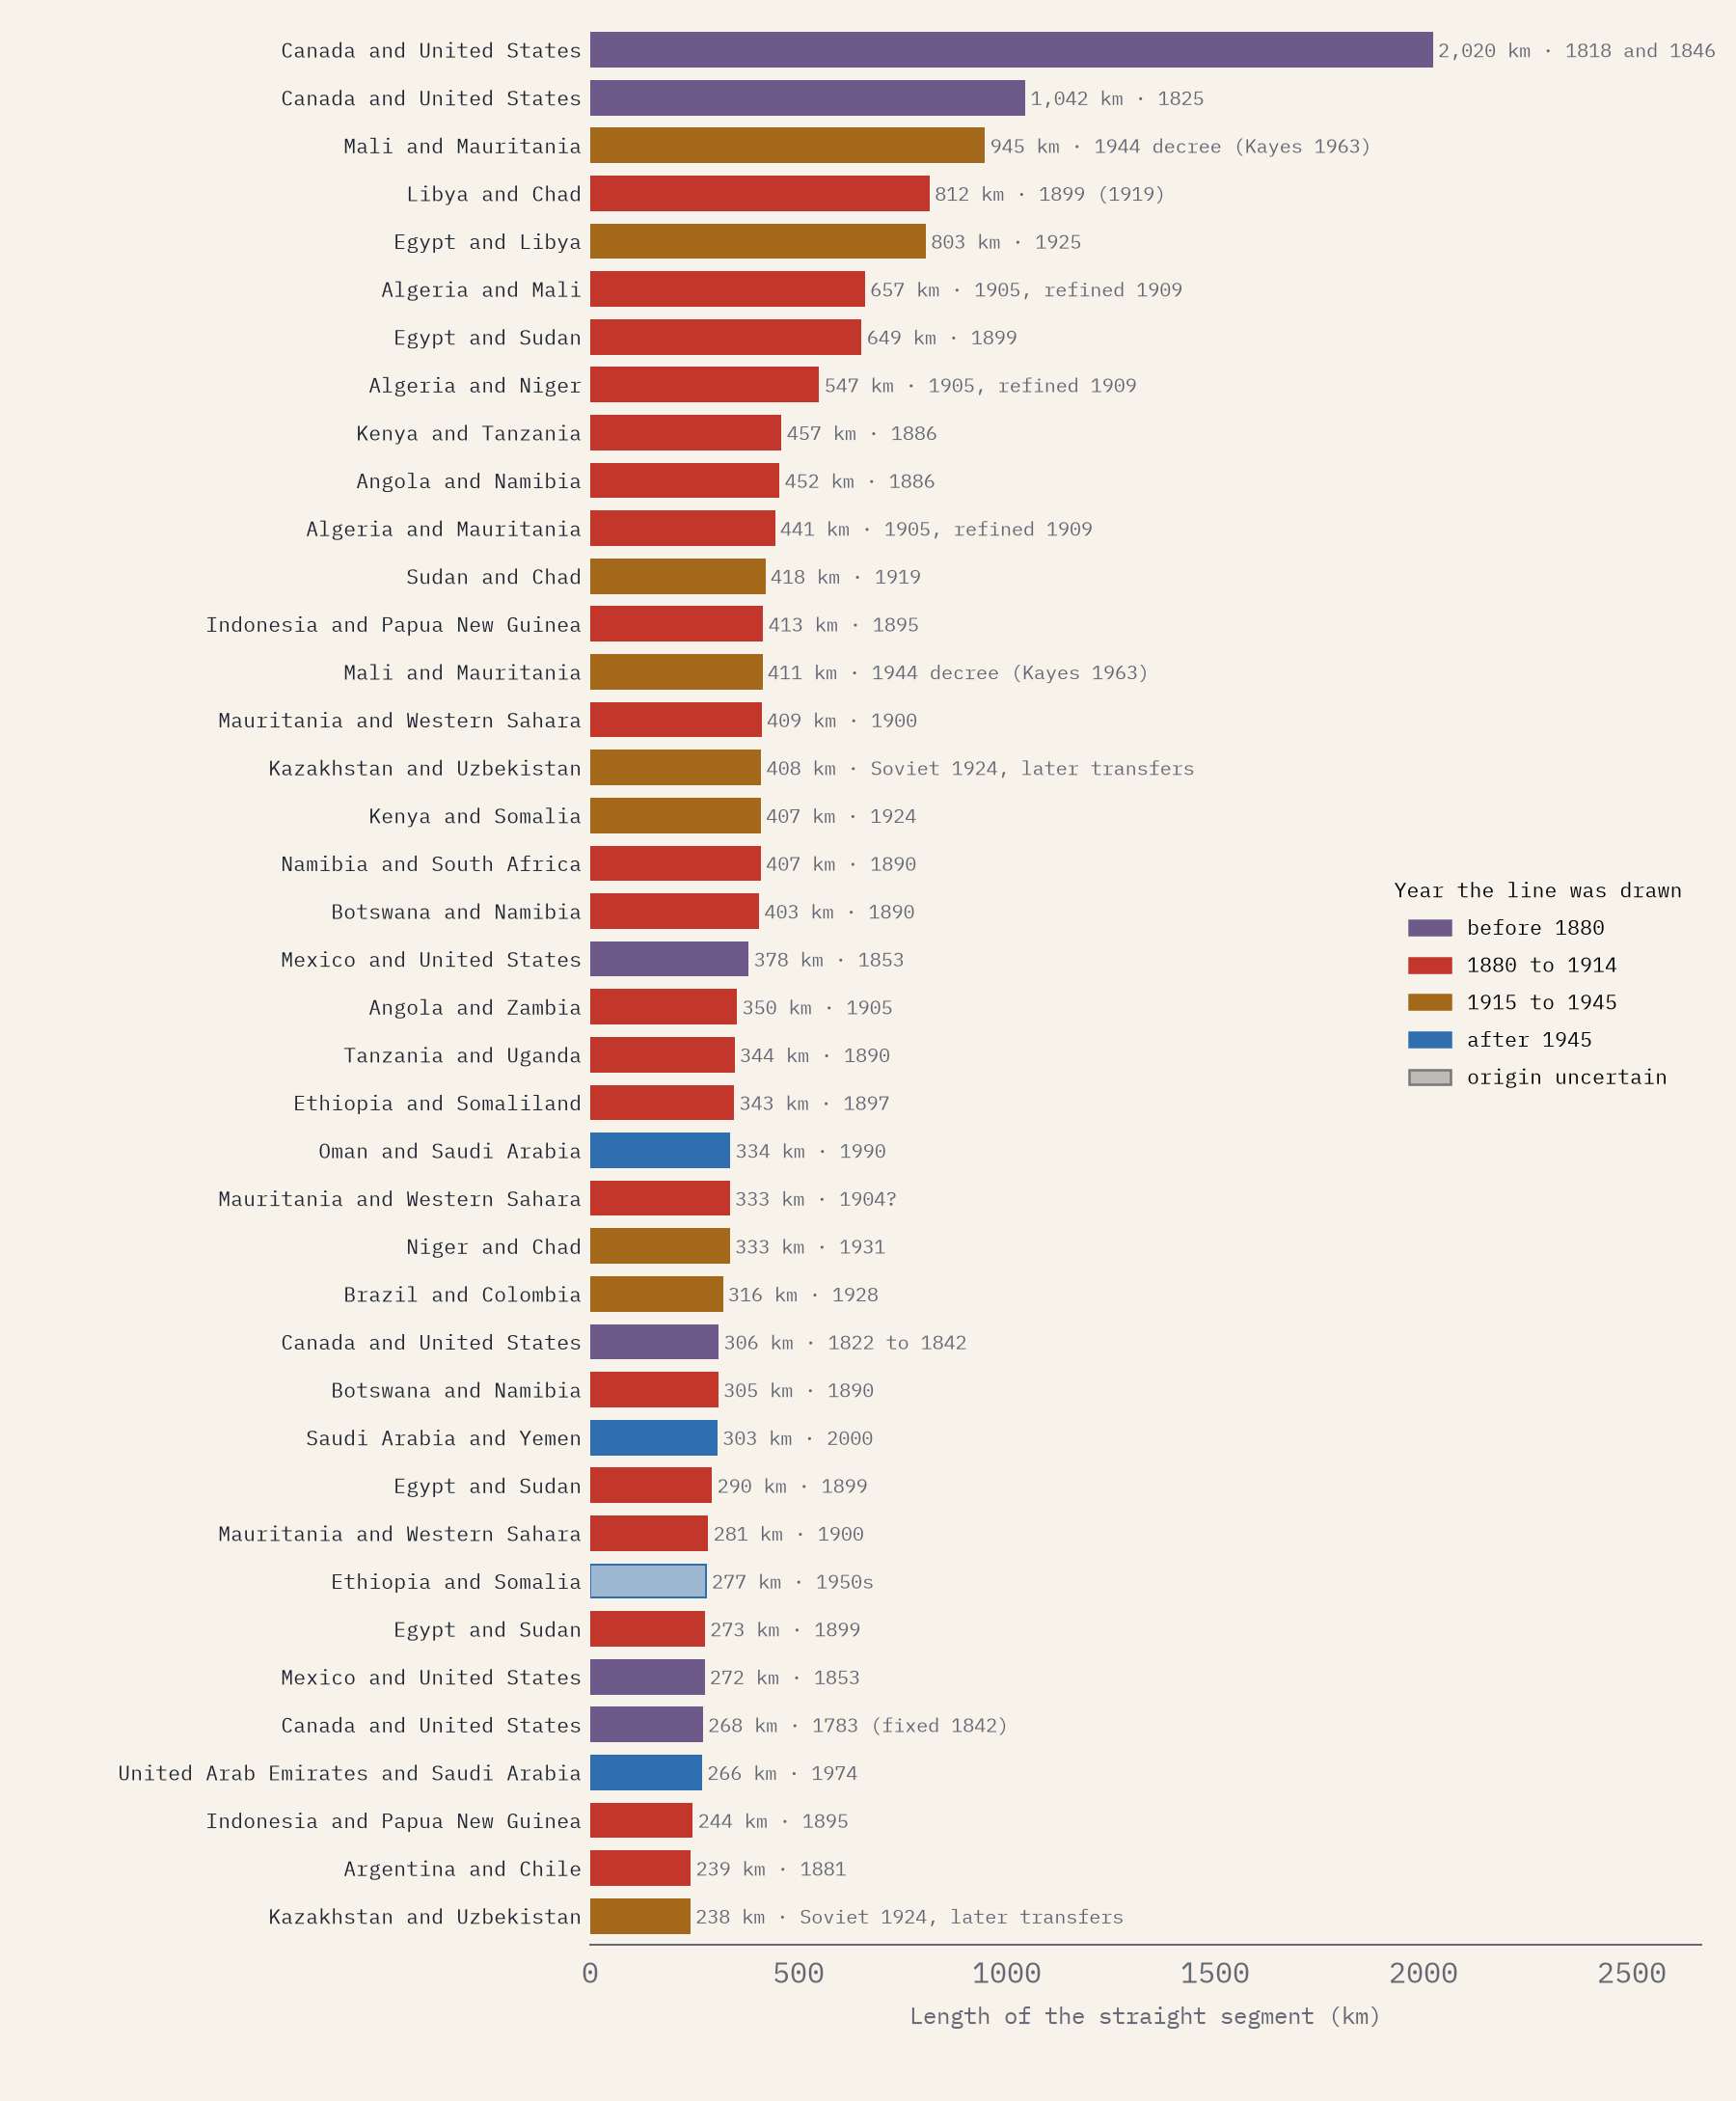
\includegraphics[width=.92\textwidth]{f_top.png}
\caption{The 40 longest straight segments, coloured by the period in which the line was set. Pale bars: origin uncertain.}\label{fig:top}\end{figure}

\begin{figure}[tbp]\centering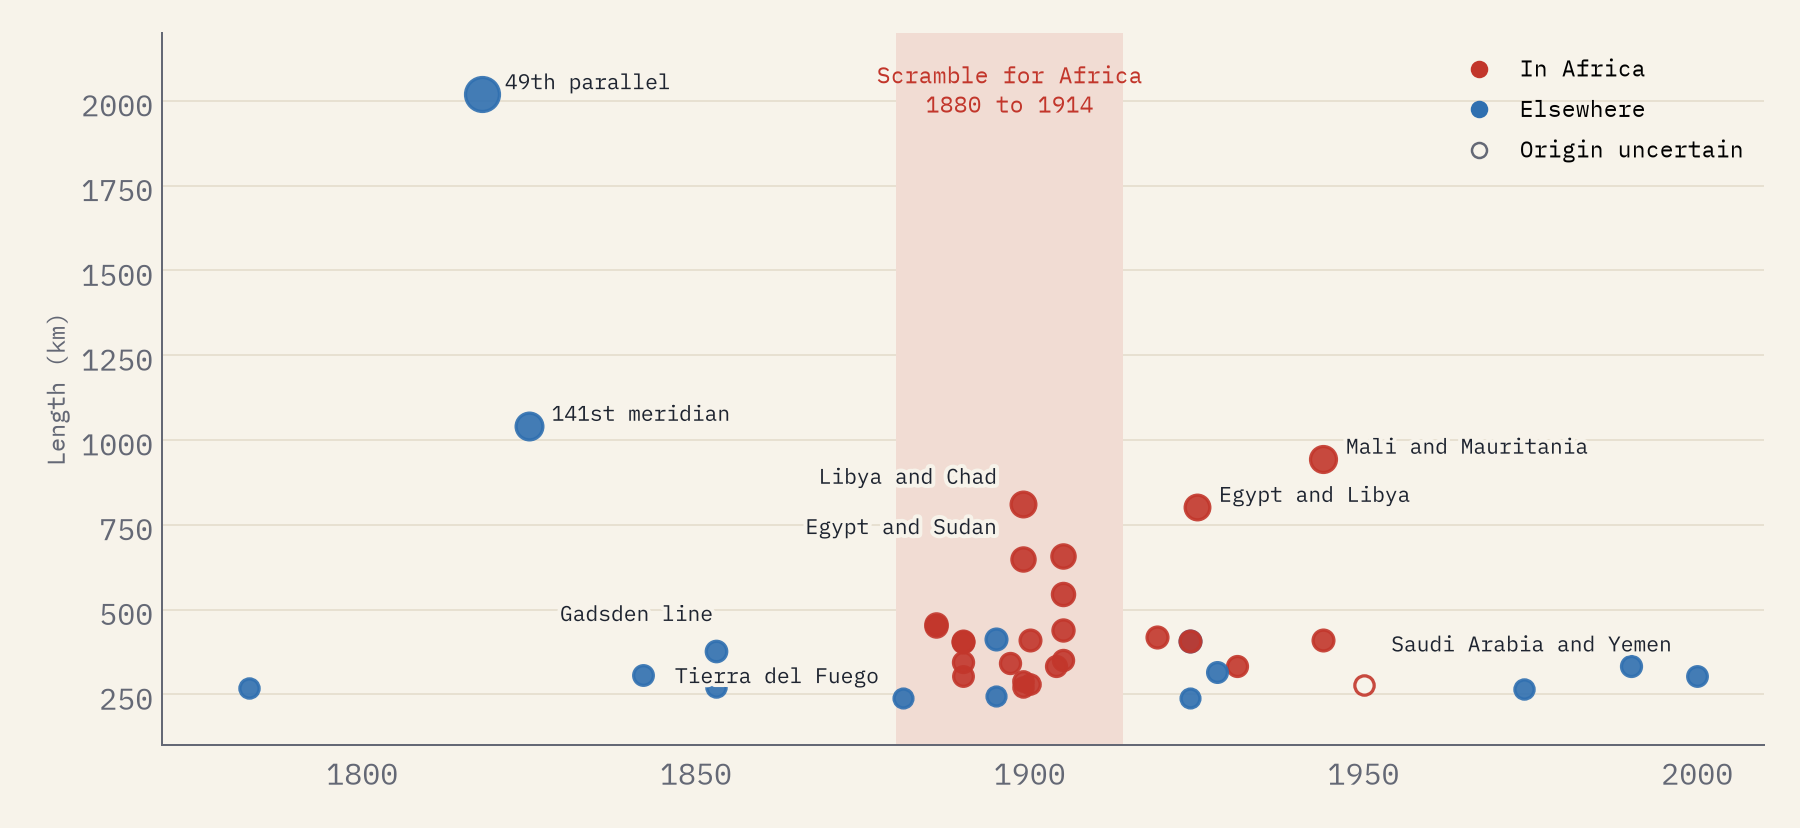
\includegraphics[width=.92\textwidth]{f_timeline.png}
\caption{Year each of the longest straight lines was set, against its length. Hollow: origin uncertain.}\label{fig:time}\end{figure}

{\footnotesize\setlength{\tabcolsep}{3pt}\begin{longtable}{r>{\raggedright\arraybackslash}p{2.6cm}r>{\raggedright\arraybackslash}p{1.5cm}>{\raggedright\arraybackslash}p{5.2cm}>{\raggedright\arraybackslash}p{3.1cm}l}\caption{The 40 longest straight segments and the agreements that set them. Confidence: high, a well-known treaty set this line; medium, the treaty is known but the instrument or date for this stretch is less certain; low, an administrative line or uncertain origin. Sources are listed for each line in data/straight\_segments.csv.}\label{tab:top}\\\toprule \# & Border & km & Year & Agreement & Agreed by & Conf.\\\midrule\endfirsthead\toprule \# & Border & km & Year & Agreement & Agreed by & Conf.\\\midrule\endhead
1 & Canada and United States & 2,020 & 1818 and 1846 & Convention of 1818 (east of the Rocky Mountains) and Oregon Treaty (west of them) & United Kingdom, United States & high\\
2 & Canada and United States & 1,042 & 1825 & Anglo-Russian Convention of St Petersburg & Russian Empire, United Kingdom & high\\
3 & Mali and Mauritania & 945 & 1944 decree (Kayes 1963) & French colonial decree moving the line between French Sudan and Mauritania (first drawn in 1913) & France (colonial decree); then Mali and Mauritania & medium\\
4 & Libya and Chad & 812 & 1899 (1919) & Anglo-French Declaration (1899), as interpreted in the Anglo-French Convention of 1919 & France, United Kingdom & high\\
5 & Egypt and Libya & 803 & 1925 & Italo-Egyptian boundary agreement & Egypt, Italy (with the United Kingdom) & high\\
6 & Algeria and Mali & 657 & 1905, refined 1909 & Agreement between the Commandant of Upper Senegal and Niger and the Military Commander of the Oasis territory (French Algeria), further defined by the Niamey Convention of 1909 & France (between its own colonial administrations) & medium\\
7 & Egypt and Sudan & 649 & 1899 & Anglo-Egyptian Condominium Agreement & Egypt, United Kingdom & high\\
8 & Algeria and Niger & 547 & 1905, refined 1909 & Agreement between the Commandant of Upper Senegal and Niger and the Military Commander of the Oasis territory (French Algeria), further defined by the Niamey Convention of 1909 & France (between its own colonial administrations) & medium\\
9 & Kenya and Tanzania & 457 & 1886 & Anglo-German Agreement & Germany, United Kingdom & high\\
10 & Angola and Namibia & 452 & 1886 & Portuguese-German Declaration & Germany, Portugal & high\\
11 & Algeria and Mauritania & 441 & 1905, refined 1909 & Agreement between the Commandant of Upper Senegal and Niger and the Military Commander of the Oasis territory (French Algeria), further defined by the Niamey Convention of 1909 & France (between its own colonial administrations) & medium\\
12 & Sudan and Chad & 418 & 1919 & Anglo-French Convention (following the 1899 Declaration) & France, United Kingdom & medium\\
13 & Indonesia and Papua New Guinea & 413 & 1895 & Anglo-Dutch boundary treaty & Netherlands, United Kingdom & medium\\
14 & Mali and Mauritania & 411 & 1944 decree (Kayes 1963) & French colonial decree moving the line between French Sudan and Mauritania (first drawn in 1913) & France (colonial decree); then Mali and Mauritania & medium\\
15 & Mauritania and Western Sahara & 409 & 1900 & Franco-Spanish Convention of Paris & France, Spain & high\\
16 & Kazakhstan and Uzbekistan & 408 & Soviet 1924, later transfers & Soviet national-territorial delimitation between the Kazakh and Uzbek (Karakalpak) republics, with transfers in 1936, 1956 and 1963 & Soviet Union (between its own republics); then Kazakhstan and Uzbekistan & medium\\
17 & Kenya and Somalia & 407 & 1924 & Anglo-Italian Treaty ceding Jubaland to Italy & Italy, United Kingdom & high\\
18 & Namibia and South Africa & 407 & 1890 & Anglo-German Agreement (Heligoland-Zanzibar Treaty) & Germany, United Kingdom & high\\
19 & Botswana and Namibia & 403 & 1890 & Anglo-German Agreement (Heligoland-Zanzibar Treaty) & Germany, United Kingdom & high\\
20 & Mexico and United States & 378 & 1853 & Gadsden Purchase (Treaty of La Mesilla) & Mexico, United States & high\\
21 & Angola and Zambia & 350 & 1905 & Arbitral award of King Victor Emmanuel III of Italy on the western limits of Barotseland & Portugal, United Kingdom (arbitrated by Italy) & medium\\
22 & Tanzania and Uganda & 344 & 1890 & Anglo-German Agreement (Heligoland-Zanzibar Treaty) & Germany, United Kingdom & high\\
23 & Ethiopia and Somaliland & 343 & 1897 & Anglo-Ethiopian Treaty (Rennell Rodd) & Ethiopia, United Kingdom & high\\
24 & Oman and Saudi Arabia & 334 & 1990 & Saudi-Omani boundary agreement & Oman, Saudi Arabia & medium\\
25 & Mauritania and Western Sahara & 333 & 1904? & Franco-Spanish conventions (1900, extended north in 1904) & France, Spain & medium\\
26 & Niger and Chad & 333 & 1931 & Memorandum No. 2268 transferring Tibesti from French West Africa to French Equatorial Africa & France (between its own colonial administrations) & medium\\
27 & Brazil and Colombia & 316 & 1928 & Brazil-Colombia boundary treaty & Brazil, Colombia & medium\\
28 & Canada and United States & 306 & 1822 to 1842 & Boundary commissions under the Treaty of Ghent, confirmed by the Webster-Ashburton Treaty & United Kingdom, United States & medium\\
29 & Botswana and Namibia & 305 & 1890 & Anglo-German Agreement (Heligoland-Zanzibar Treaty) & Germany, United Kingdom & high\\
30 & Saudi Arabia and Yemen & 303 & 2000 & Treaty of Jeddah & Saudi Arabia, Yemen & high\\
31 & Egypt and Sudan & 290 & 1899 & Anglo-Egyptian Condominium Agreement & Egypt, United Kingdom & high\\
32 & Mauritania and Western Sahara & 281 & 1900 & Franco-Spanish Convention of Paris & France, Spain & medium\\
33 & Ethiopia and Somalia & 277 & 1950s & Provisional Administrative Line (British), drawn after the Ogaden and Haud returned to Ethiopia; the Italo-Ethiopian convention of 1908 was never demarcated & United Kingdom (provisional line); Ethiopia and Italy in 1908 & low\\
34 & Egypt and Sudan & 273 & 1899 & Anglo-Egyptian Condominium Agreement & Egypt, United Kingdom & high\\
35 & Mexico and United States & 272 & 1853 & Gadsden Purchase (Treaty of La Mesilla) & Mexico, United States & high\\
36 & Canada and United States & 268 & 1783 (fixed 1842) & Treaty of Paris (1783), line fixed by the Webster-Ashburton Treaty & United Kingdom, United States & high\\
37 & United Arab Emirates and Saudi Arabia & 266 & 1974 & Treaty of Jeddah (text long unpublished; the line drawn is approximate) & Saudi Arabia, United Arab Emirates & medium\\
38 & Indonesia and Papua New Guinea & 244 & 1895 & Anglo-Dutch boundary treaty & Netherlands, United Kingdom & medium\\
39 & Argentina and Chile & 239 & 1881 & Boundary Treaty of 1881 & Argentina, Chile & high\\
40 & Kazakhstan and Uzbekistan & 238 & Soviet 1924, later transfers & Soviet national-territorial delimitation between the Kazakh and Uzbek (Karakalpak) republics, with transfers in 1936, 1956 and 1963 & Soviet Union (between its own republics); then Kazakhstan and Uzbekistan & medium\\
\bottomrule\end{longtable}}

\subsection{Rivers and mountains}
The borders with most river length are China and Russia (2,857 km, 80.6\% of the border, on the Amur, Argun and Ussuri), Canada and the United States, Argentina and Paraguay, and Mexico and the United States (Figure~\ref{fig:rm}). The borders with most mountain length are Argentina and Chile (3,881 km), China and India, and Afghanistan and Pakistan. Water shares range from 19.4\% to 23.6\% across the settings tested, and mountain shares from 11.0\% to 32.4\%.

\begin{figure}[tbp]\centering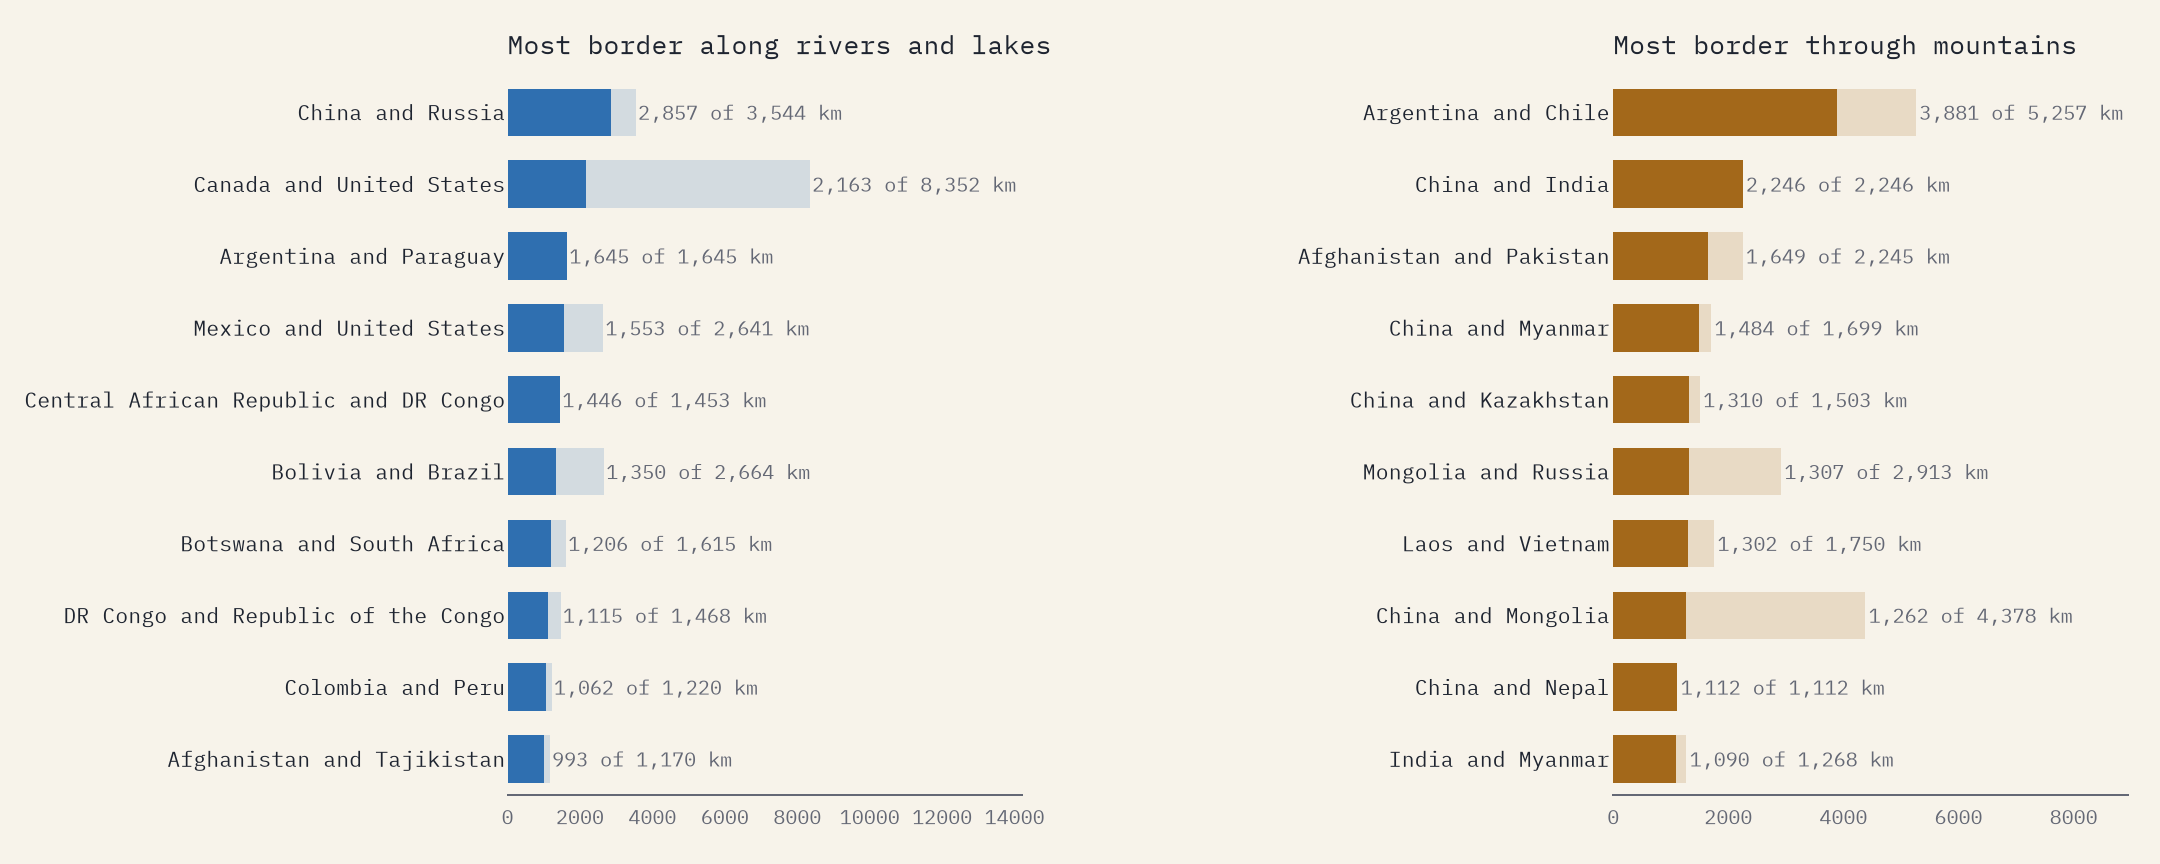
\includegraphics[width=\textwidth]{f_rivers.png}
\caption{The ten borders with the most river or lake length and the most mountain length.}\label{fig:rm}\end{figure}

\subsection{Sensitivity and map scale}
With a 50 km minimum the world straight share ranges from 18.0\% to 24.0\% across tolerances; with a 100 km minimum it falls to 13.5\% to 15.1\%, and only the loosest combination (25 km within 2 km) reaches 51.4\%, because it admits ordinary irregular border. Map scale matters more (Figure~\ref{fig:scale}): the same test finds 25.4\% straight on Natural Earth's 1:50 million lines and 83.6\% on the 1:110 million lines, where generalisation turns winding borders into chains of long straight edges. Even the 1:10 million lines smooth some detail, so the straight share on the ground is likely a little lower than measured here.

\begin{figure}[tbp]\centering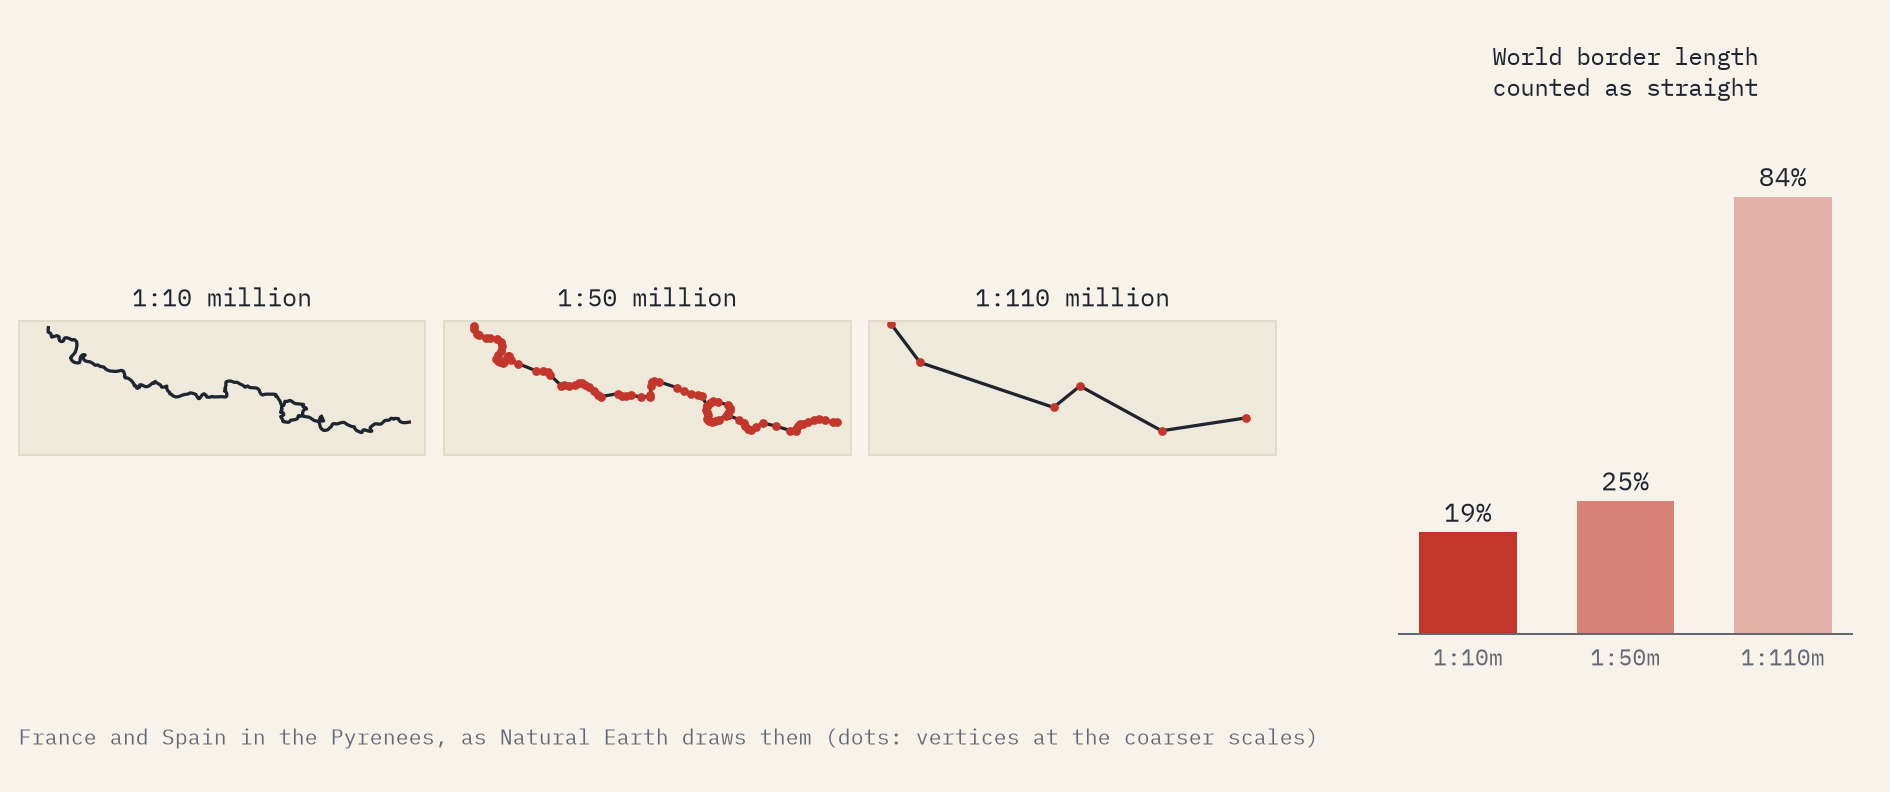
\includegraphics[width=\textwidth]{f_scale.png}
\caption{Left: the border between France and Spain at three Natural Earth scales. Right: share of world border length counted as straight at each scale, same method and settings.}\label{fig:scale}\end{figure}

\section{Limitations}
First, the measurement is of a map, not the ground: Natural Earth's lines are generalised for 1:10 million and may depart from surveyed boundaries by hundreds of metres or more, and short straight sections (under 50 km) are not counted. Second, the river class depends on which rivers Natural Earth maps; small border streams are missed, so the water share is a lower bound and some water borders fall into other. Third, the mountain class describes terrain, not whether the line follows a crest or watershed; a finer elevation model and a drainage analysis would be needed for that. Fourth, the treaty table is compiled by hand from secondary sources; dates are the year a line was first set in roughly its present form, and later adjustments, demarcations and disputes are summarised briefly. I mark 1 of 40 attributions as low confidence (the provisional line between Ethiopia and Somalia) and 18 as medium, mainly French colonial administrative limits and Soviet internal lines whose instruments are documented but less well known. Fifth, the categories are not exclusive in reality (a straight line may cross a lake, a river may run through mountains), and the priority order shapes the shares. Sixth, a border's shape says nothing by itself about its legitimacy or its effects; straight lines were often drawn without regard to the people living on them, but irregular colonial lines could be just as arbitrary.

\section{Conclusion}
About a fifth of the world's land border is ruler-straight, and more than half of that is in Africa. But the claim that Africa's borders are the straightest holds only by quantity: by share of length North America is straighter, because of the long parallel and meridian between Canada and the United States. The longest straight lines were overwhelmingly drawn by or with European powers, most of them between 1880 and 1914, but the list also includes American, Arabian and Soviet lines, and some of the straightest borders in the Sahara began as lines between one empire's own colonies. The data and the treaty table are open for correction and reuse.

\section*{Data and code availability}
The interactive map is at \url{https://maps.tristanhotham.com/straight-borders/}. Data and code are at \url{https://github.com/Tristan-Hotham/straight-borders} and archived with this paper at \url{https://doi.org/10.5281/zenodo.23847974}. Natural Earth and ETOPO5 are public domain. Code is MIT; text, figures and derived data are CC BY 4.0.

\section*{AI statement}
I wrote the text, with drafting and editing assistance from Claude (Anthropic), which also helped prepare the analysis code. I reviewed and checked all text and results.

\begin{thebibliography}{12}
\bibitem[Alesina et al.(2011)]{alesina2011} Alesina, A., Easterly, W. and Matuszeski, J. (2011) Artificial states. \emph{Journal of the European Economic Association}, 9(2), 246 to 277.
\bibitem[Barbour(1961)]{barbour1961} Barbour, K. M. (1961) A geographical analysis of boundaries in inter-tropical Africa. In Barbour, K. M. and Prothero, R. M. (eds) \emph{Essays on African Population}. London: Routledge and Kegan Paul.
\bibitem[Biger(1995)]{biger1995} Biger, G. (ed.) (1995) \emph{The Encyclopedia of International Boundaries}. New York: Facts on File.
\bibitem[Brownlie(1979)]{brownlie1979} Brownlie, I. (1979) \emph{African Boundaries: A Legal and Diplomatic Encyclopaedia}. London: C. Hurst for the Royal Institute of International Affairs.
\bibitem[ICJ(1994)]{icj1994} International Court of Justice (1994) \emph{Territorial Dispute (Libyan Arab Jamahiriya/Chad)}, Judgment of 3 February 1994. ICJ Reports 1994.
\bibitem[Kapos et al.(2000)]{kapos2000} Kapos, V., Rhind, J., Edwards, M., Price, M. F. and Ravilious, C. (2000) Developing a map of the world's mountain forests. In Price, M. F. and Butt, N. (eds) \emph{Forests in Sustainable Mountain Development}. Wallingford: CABI.
\bibitem[Michalopoulos and Papaioannou(2016)]{michalopoulos2016} Michalopoulos, S. and Papaioannou, E. (2016) The long-run effects of the Scramble for Africa. \emph{American Economic Review}, 106(7), 1802 to 1848.
\bibitem[Natural Earth(2026)]{naturalearth} Natural Earth (2026) Admin 0 boundary lines, countries, rivers and lake centre lines, lakes and physical regions, version 5.2.0-pre. Public domain. \url{https://www.naturalearthdata.com/}
\bibitem[NGDC(1988)]{etopo5} National Geophysical Data Center (1988) \emph{ETOPO5: 5-minute gridded elevations of the Earth}. Boulder: NOAA. Public domain.
\bibitem[Prescott and Triggs(2008)]{prescott2008} Prescott, V. and Triggs, G. D. (2008) \emph{International Frontiers and Boundaries: Law, Politics and Geography}. Leiden: Martinus Nijhoff.
\end{thebibliography}
\end{document}
